\documentclass[a4paper,11pt,DIV20,BCOR0mm]{scrartcl}
\usepackage[utf8]{inputenc}
\usepackage[francais]{babel}
\usepackage[T1]{fontenc}
\usepackage{amsmath}
\usepackage{amssymb}
\usepackage{color}
\usepackage{textcomp}
\usepackage[official]{eurosym}
\usepackage{enumitem}
\usepackage{numprint}
\usepackage{graphicx}
\usepackage{xifthen}
\usepackage{pifont}
%\usepackage{xlop}
\usepackage{subfig}
\usepackage{cellspace,stmaryrd}
\usepackage[french]{varioref}
\usepackage{pstricks,pst-circ,pstricks-add,pst-plot,pst-math}
%\usepackage{pst-all,pst-tree,pst-3dplot}
\RequirePackage[amsmath,thmmarks,hyperref,framed]{ntheorem}
\usepackage{mathrsfs}

% ==================================================
% Intervalles
% ==================================================
\newcommand{\intervalle}[4]{\mathopen{#1}#2\mathpunct{};#3\mathclose{#4}}
\newcommand{\intff}[2]{\intervalle{[}{#1}{#2}{]}}
\newcommand{\intof}[2]{\intervalle{]}{#1}{#2}{]}}
\newcommand{\intfo}[2]{\intervalle{[}{#1}{#2}{[}}
\newcommand{\intoo}[2]{\intervalle{]}{#1}{#2}{[}}
\newcommand{\intn}[2]{\intervalle{\llbracket}{#1}{#2}{\rrbracket}}
\newcommand{\bigintervalle}[4]{\bigl{#1}#2\mathpunct{};#3\bigr{#4}}
\newcommand{\bigintff}[2]{\bigintervalle{[}{#1}{#2}{]}}
\newcommand{\bigintof}[2]{\bigintervalle{]}{#1}{#2}{]}}
\newcommand{\bigintfo}[2]{\bigintervalle{[}{#1}{#2}{[}}
\newcommand{\bigintoo}[2]{\bigintervalle{]}{#1}{#2}{[}}
\newcommand{\bigintn}[2]{\bigintervalle{\llbracket}{#1}{#2}{\rrbracket}}
\newcommand{\Bigintervalle}[4]{\Bigl{#1}#2\mathpunct{};#3\Bigr{#4}}
\newcommand{\Bigintff}[2]{\Bigintervalle{[}{#1}{#2}{]}}
\newcommand{\Bigintof}[2]{\Bigintervalle{]}{#1}{#2}{]}}
\newcommand{\Bigintfo}[2]{\Bigintervalle{[}{#1}{#2}{[}}
\newcommand{\Bigintoo}[2]{\Bigintervalle{]}{#1}{#2}{[}}
\newcommand{\Bigintn}[2]{\Bigintervalle{\llbracket}{#1}{#2}{\rrbracket}}
\newcommand{\biggintervalle}[4]{\biggl{#1}#2\mathpunct{};#3\biggr{#4}}
\newcommand{\biggintff}[2]{\biggintervalle{[}{#1}{#2}{]}}
\newcommand{\biggintof}[2]{\biggintervalle{]}{#1}{#2}{]}}
\newcommand{\biggintfo}[2]{\biggintervalle{[}{#1}{#2}{[}}
\newcommand{\biggintoo}[2]{\biggintervalle{]}{#1}{#2}{[}}
\newcommand{\biggintn}[2]{\biggintervalle{\llbracket}{#1}{#2}{\rrbracket}}
\newcommand{\Biggintervalle}[4]{\Biggl{#1}#2\mathpunct{};#3\Biggr{#4}}
\newcommand{\Biggintff}[2]{\Biggintervalle{[}{#1}{#2}{]}}
\newcommand{\Biggintof}[2]{\Biggintervalle{]}{#1}{#2}{]}}
\newcommand{\Biggintfo}[2]{\Biggintervalle{[}{#1}{#2}{[}}
\newcommand{\Biggintoo}[2]{\Biggintervalle{]}{#1}{#2}{[}}
\newcommand{\Biggintn}[2]{\Biggintervalle{\llbracket}{#1}{#2}{\rrbracket}}

\newcommand{\pt}{.}
\newcommand{\et}{\text{ et }}
\newcommand{\si}{\text{ si }}
\newcommand{\tq}{\text{ tq }}
\newcommand{\sinon}{\text{ sinon }}
\newcommand{\avec}{\text{ avec }}
\def\pour{\text{~pour~}}

\newenvironment{enumeratecol}[1][2]{\begin{multicols}{#1}\begin{enumerate}}{\end{enumerate}\end{multicols}}


\newcommand{\set}[1]{\left\{#1\right\}}


%\newtheorem{theoreme}{Théorème}
%\newtheorem{axiome}{Axiome}
\newtheorem*{proprieteadmise}{Propriété (admise)}
%\newtheorem*{demonstration}{Démonstration}
\newtheorem*{notation}{Notation}
\newtheorem*{application}{Application}
\newtheorem*{consequence}{Conséquence}
\newtheorem{roc}{Restitution organisée de connaissances.}


\theoremstyle{plain}
\theoremheaderfont{\normalfont\bfseries}
\theorembodyfont{\normalfont}
\theoremseparator{.}
\newtheorem{exercice}{Exercice}
\newtheorem{cours}{Question de cours}
\newtheorem{probleme}{Problème}

\theoremstyle{plain}
\theoremheaderfont{\normalfont\bfseries}
\theorembodyfont{\normalfont}
\theoremseparator{.}
\newtheorem*{rappel}{Rappel}
\newtheorem{exemple}{Exemple}
\newtheorem*{contreexemple}{Contre-exemple}
\newtheorem{remarque}{Remarque}
\newtheorem*{interpretation}{Interprétation}
\newtheorem*{convention}{Convention}
\newtheorem*{vocabulaire}{vocabulaire}

\theoremheaderfont{\sc}\theorembodyfont{\upshape}
\theoremstyle{nonumberplain}
\theoremseparator{ : }
%\theoremsymbol{\rule{1ex}{1ex}}
\theoremsymbol{\ensuremath\square}
\newtheorem{demonstration}{D\'emonstration}



\usepackage[S]{thmbox}
\newtheorem[S]{theoreme}{Théorème}
\newtheorem[S]{propriete}{Propriété}
\newtheorem[S]{axiome}{Axiome}
\newtheorem[S]{methode}{Méthode de résolution}
\newtheorem[L]{definition}{Définition}

\newcommand{\defi}[1]{
\begin{definition}
#1
\end{definition}
}

\newcommand{\theo}[1]{
\begin{theoreme}
#1
\end{theoreme}
}

\newcommand{\demo}[1]{
\begin{demonstration}
#1
\end{demonstration}
}


%-------------------------------------------------
%         TYPOGRAPHIE
%-------------------------------------------------
\newcommand{\celsius}{\,\degres\textrm{C}}


%-------------------------------------------------
%         SCOLAIRE
%-------------------------------------------------
\newcommand{\trou}[1]{\textcolor{white}{#1}}
\newcommand{\prof}[1]{\textcolor{blue}{#1}}
\newcommand{\exercices}[1]{\begin{flushright}\textbf{Exercices : }#1\end{flushright}}

\newcommand{\np}[1]{\numprint{#1}}

\newcommand{\place}[1]{
\vfill\begin{center}
< #1>
\end{center}
\vfill
}

\newif\ifeleve
\def\ac#1{\ifeleve%
\setbox1\hbox{#1}%
\lower2pt\hbox to \wd1{\dotfill}%
\else#1\fi}

\newcommand{\croi}{% croissante
\unitlength=1cm
\begin{minipage} {1cm}%pour centrer verticalement f(x)
\begin{picture}(1,1) % dessin de 2 X 2
\put(0,0){\vector(1,1){1}} % 1 à partir (0,0) direction (1,1)
\end{picture}
\end{minipage}
}
\newcommand{\dec}{%décroissante
\unitlength=1cm
\begin{minipage} {1cm}%pour centrer verticalement f(x)
\begin{picture}(1,1) % dessin de 2 X 2
\put(0,1){\vector(1,-1){1}}
\end{picture}
\end{minipage}
} 

\newcommand{\tauxfxh}[3]{\dfrac{#1(#2+#3)-#1(#2)}{#3}}

\newcounter{QCM}
\setcounter{QCM}{1}
\newcommand{\question}[1]{{\item[Question \arabic{QCM}]\addtocounter{QCM}{1}#1}}
\newcommand{\choix}[3]{
\[
 \begin{tabular}{p{5cm}p{5cm}p{5cm}}
  \textbf{a) }#1.&\textbf{b) }#2.&\textbf{c) }#3.
 \end{tabular}
\]
}

%-------------------------------------------------
%         GEOMETRIE
%-------------------------------------------------
\newcommand{\vect}{\overrightarrow}
\newcommand{\norme}[1]{\|#1\|}
\newcommand{\Norme}[1]{\left\|#1\right\|}
\newcommand{\Oijk}{(O,\vect{i},\vect{j},\vect{k})}
\newcommand{\Oij}{(O,\vect{i},\vect{j})}
\newcommand{\Ouv}{(O,\vect{u},\vect{v})}
\newcommand{\bary}{\mathrm{Bar}}

%-------------------------------------------------
%         FONCTIONS
%-------------------------------------------------
\newcommand{\donne}{\mapsto}
\newcommand{\dx}{\mathrm{d}x}
\newcommand{\dt}{\mathrm{d}t}
\newcommand{\intab}{\int_{a}^{b}}
%-------------------------------------------------
%         PROBA
%-------------------------------------------------
\newcommand{\barre}[1]{\overline{#1}}

%-------------------------------------------------
%         ALGEBRE LINEAIRE
%-------------------------------------------------
\newcommand{\rg}{\text{rg}}
\newcommand{\tr}{\text{tr}}
\renewcommand{\Im}{\text{Im}}
\newcommand{\Vect}{\text{Vect}}
\newcommand{\LL}{\mathcal{L}}
\newcommand{\FF}{\mathcal{F}}
\newcommand{\MM}{\mathcal{M}}
\newcommand{\transpose}{{}^{t}}
%\newcommand{\ker}{\text{ker}}
\newcommand{\coordo}[2]{
\begin{pmatrix}
#1 \\ #2
\end{pmatrix}
}

%-------------------------------------------------
%         ARITHMETIQUE
%-------------------------------------------------
\newcommand{\congru}{\equiv}

%-------------------------------------------------
%         NOMBRES COMPLEXES
%-------------------------------------------------
\newcommand{\e}{\mathrm{e}}
\newcommand{\ii}{\mathrm{i}}
\newcommand{\ei}[1]{\mathrm{e}^{\ii#1}}
\newcommand{\C}{\mathbb{C}}
\newcommand{\U}{\mathbb{U}}
\newcommand{\re}[1]{\mathrm{Re}(#1)}
\newcommand{\im}[1]{\mathrm{Im}(#1)}
\newcommand{\conj}[1]{\overline{#1}}
\newcommand{\abs}[1]{\left\lvert#1\right\rvert}
\renewcommand{\arg}[1]{\mathrm{Arg}(#1)}

\newcommand{\pparmin}[2]{\binom{#2}{#1}}
\newcommand{\Pparmin}[2]{\dbinom{#2}{#1}}

\newcommand{\R}{\mathbb{R}}
\newcommand{\K}{\mathbb{K}}
\newcommand{\N}{\mathbb{N}}
\newcommand{\Z}{\mathbb{Z}}
\newcommand{\D}{\mathbb{D}}
\newcommand{\Q}{\mathbb{Q}}
\newcommand{\rond}{\circ}
\newcommand{\repereoij}{repère orthonormal $(O,\vect{i},\vect{j})$}
\newcommand{\repereoijdirect}{repère orthonormal direct $(O,\vect{i},\vect{j})$}
\newcommand{\accoladedouble}[2]{\left\{\begin{array}{ll}#1\\#2\end{array}\right.}
\newcommand{\soitlasuite}[4]{Soit $(#1)$ la suite définie par $\accoladedouble{#2}{#3\text{ pour tout $#4$}}$}
\newcommand{\coordvect}[2]{\left(\begin{array}{c}#1\\#2\end{array}\right)}
\newcommand{\baremeexo}[1]{\marginpar{\textbf{(#1)}}}
\newcommand{\baremeque}[1]{\marginpar{(#1)}}
\newcommand{\bq}[1]{\marginpar{\textcolor{red}{(#1)}}}


\newcommand{\less}{\leqslant}
\newcommand{\more}{\geqslant}
\newcommand{\equi}{\Longleftrightarrow}
\newcommand{\implique}{\Rightarrow}
\newcommand{\equidef}{\stackrel{def}{\Longleftrightarrow}}
\newcommand{\ssi}{\Longleftrightarrow}
\newcommand{\eqdef}{\stackrel{def}{=}}
\newcommand{\egaldef}{\stackrel{\tiny{def}}{=}}
\newcommand{\egalnot}{\stackrel{\tiny{notation}}{=}}
\newcommand{\latin}[1]{\emph{#1}}
\newcommand{\negl}[1]{\underset{\text{\tiny{$#1$}}}{\ll}}

\newcommand{\limsuite}{\displaystyle\lim_{n\to+\infty}}

% Partie à ommettre en première lecture
\newcommand{\optionnel}[1]{\noindent\hrulefill \rotatebox{180}{\ding{72}\ding{72}\ding{72}} \hrulefill #1 \noindent\hrulefill \ding{72}\ding{72}\ding{72} \hrulefill}
% En tête et pieds custom
\usepackage{fancyhdr}
\pagestyle{fancy}
\lhead{\today}
\rhead{Cours}		
\lfoot{\tiny{vg}}
\cfoot{}
\rfoot{\tiny{Lycée Émile Loubet, Valence}}


% de Dupuy de lome
%\newcommand{\norme}[1]{\left\lVert\ifempty{#1}{\dotpourvariable}{#1}\right\rVert}
\newcommand{\bignorme}[1]{\bigl\lVert#1\bigr\rVert}
\usepackage{hyperref}
\rhead{Septembre 2014}
\chead{}
\lhead{Généralités sur les suites, axiome de récurrence}
\lfoot{\tiny{vg}}
\cfoot{\thepage}
\rfoot{\tiny{Julie-Victoire Daubié, Argenteuil, TS1}}
\begin{document}

\section{Définitions et rappels}
\subsection{Qu'est-ce qu'une suite ?}
\begin{definition}[Suite numérique réelle]
 Une suite numérique réelle $(u_n)_{n\in\N}$ est une fonction de $\N$ dans $\R$, autrement dit
à chaque entier $n$ elle fait correspondre un unique réel $u(n)$, habituellement noté $u_n$.
\end{definition}
On considère aussi des suites définies sur $\N^*$, voire sur des parties de $\N$ de
la forme $\{n\in\N,\,n\geq p\}$, avec $p\in\N$.

Vous rencontrerez 2 manières de définir une suite :
\begin{itemize}
 \item \emph{explicite}, on donne explicitement une fonction en disant par exemple : soit $(u_n)$ la suite
définie par $u_n=n^2-n+41$ pour tout $n\in\N$. Graphiquement, si on a la représentation graphique de 
la fonction on obtient facilement les termes de la suite.
\vfill
\begin{center}
 <graphique d'exemple>
\end{center}
\vfill
 \item \emph{par récurrence}, on donne le ou les premiers termes de la suite et une relation permettant
d'obtenir un terme à partir de ceux qui le précèdent. Par exemple la suite $(u_n)$ définie par
\[\left\{
\begin{array}{rcl}
 u_0&=&-1\\
 \text{ pour tout $n\in\N$, }u_{n+1}&=&\sqrt{u_n+2}
\end{array}
\right.\] 
Dans le cas le plus courant, on donne le terme initial et une relation de la forme $u_{n+1}=f(u_n)$.
Graphiquement, on peut obtenir sucessivement les termes de la suite (voir dans le manuel, exercice résolu 2
p. 21) :
\[
 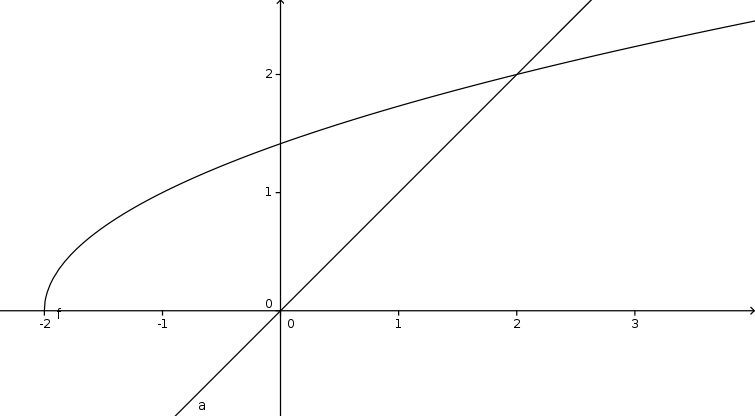
\includegraphics{recurrence}
\]
Avec la calculatrice, on peut calculer rapidement les valeurs approchées des termes successifs avec la touche \og ANS\fg (casio, de l'anglais answer)
ou \og Rép\fg{} (TI version française).
On peut aussi utiliser l'algorithme :
\begin{center}
\begin{tabular}{|p{2.5cm}p{6cm}|}\hline 
Variables:&$i$ et $n$ sont des entiers naturels.\\
& $u$ est un réel.\\
Entrée:&Demander à l'utilisateur la valeur de $n$.\\
Initialisation:& Affecter à $u$ la valeur 0.\\
Traitement:&Pour $i$ variant de 1 à $n$.\\
&\hspace{0,5cm} $\left\vert \text{Affecter à}\: u\: \text{la valeur }f(u)\right.$\\
Sortie : &Afficher $u$.\\ \hline
\end{tabular} 
\end{center}
\end{itemize}


\begin{exercice}
 Programmer l'algorithme précédent à la calculatrice, dans un programme nommé SUITEREC.
\end{exercice}


\begin{exercice}
Donner si possible une définition par récurrence et une définition explicite
pour les premiers termes de chaque suite :
\begin{itemize}
 \item 1 ; 3 ; 5 ; 7 ; 9 ; ... (suites des distances parcourues dans les secondes successives d'une chute libre dans le vide, lorsque
l'unité est la distance parcourue pendant la première seconde).
 \item 7 ; 14 ; 28 ; 56 ; ...
 \item 0 ; 1 ; 3 ; 7 ; 15 ; 31 ; 63 ; ... 
 \item -1 ; 1 ; -1 ; 1 ; -1 ; 1 ; ...
 \item 1 ; 2 ; 4 ; 8 ; 16 ; 31 ; 57 ; ... (nombre de secteurs délimités dans un cercle o\`u les cordes d'extrémités $n$ points du cercle ont été tracées).
 \item 1 ; 1,4 ; 1,41 ; 1,414 ; 1,4142 ; 1,41421 ; 1,414213 ; ...
 \item 2 ; 3 ; 5 ; 7 ; 11 ; 13 ; 17 ; ...
 \item 1 ; 1 ; 2 ; 3 ; 5 ; 8 ; 13 ; 21 ; 34 ; ...
 \item 0 ; 1 ; 3 ; 6 ; 10 ; 15 ; 21 ; ... 
\end{itemize}
Pour ce \og jeu\fg, il y a un site web : \url{http://oeis.org}.
\end{exercice}


\begin{exercice}
 Dans le manuel, 20, 21, 22 p. 30.
\end{exercice}

\begin{exemple}[Cas des sommes, notation $\sum$]
 Soit $(u_n)$ la suite définie pour tout entier naturel $n\geq1$ par :
\[
 u_n = 1+2+3+\cdots+n = \sum_{k=1}^n k.
\]
Il est utile de voir que cette \og définition\fg aux airs faussement explicites revient à la définition
par récurrence :
\[\left\{
\begin{array}{rcl}
 u_1&=&1\\
 u_{n+1}&=&u_n+n+1\text{ pour tout $n\in\N^*$.}
\end{array},
\right.\]
ou encore :
\[\left\{
\begin{array}{rcl}
 u_1&=&1\\
 u_{n}&=&u_{n-1}+n\text{ pour tout $n\geq 2$.}
\end{array}.
\right.\]
\end{exemple}

\begin{exercice}
 Programmer à la calculatrice le programme SOMME correspondant à l'algorithme suivant, 
 et décrire ce qu'affiche cet algorithme en fonction de son entrée.
 \begin{center}
\begin{tabular}{|p{2.5cm}p{6cm}|}\hline 
Variables:&$i$ et $n$ sont des entiers naturels.\\
& $S$ est un réel.\\
Entrée:&Demander à l'utilisateur la valeur de $n$.\\
Initialisation:& Affecter à $S$ la valeur 0.\\
Traitement:&Pour $i$ variant de 0 à $n$.\\
&\hspace{0,5cm} $\left\vert \text{Affecter à}\: S\: \text{la valeur }S+i\right.$\\
Sortie : &Afficher $S$.\\ \hline
\end{tabular} 
\end{center}
\end{exercice}


\begin{exercice}
 Pour les suites suivantes, écrire les 2 \og définitions\fg{} équivalentes non données parmi les
3 : avec $\cdots$, avec $\sum$, par récurrence. Calculer les 3 premiers termes de la suite.
\begin{itemize}
  \item Pour $n\geq1$, $U_n=1+\dfrac{1}{4}+\dfrac{1}{9}+\cdots+\dfrac{1}{n^2}$.
  \item Pour $n\geq1$, $V_n=\sum_{k=1}^n k^3$.
  \item $W_1=1$ et pour $n\geq2$, $W_{n}=W_{n-1}+\dfrac{1}{n}$.
  \item Pour $n\geq1$, $g_n=2n-1$ et $G_n=\sum_{k=1}^{n}g_k$.
À propos, ce texte de Galilée cité dans le sujet de Physique du bac S 2011 :
\[
 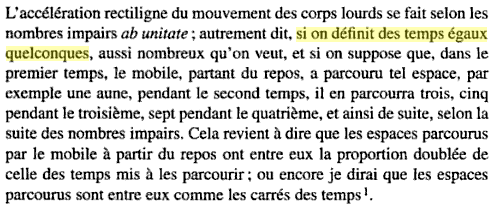
\includegraphics[width=0.5\textwidth]{galilee.png}
\]

\end{itemize}
\end{exercice}

Pour les suites arithmétiques et géométriques, le passage de la définition par
récurrence à une expression explicite est connu et simple.
\pagebreak
\subsection{Suites arithmétiques, suites géométriques}

\begin{theoreme}
Soit $(u_n)_{n\in\N}$ une suite, $a$, $q$ et $r$ des réels.
On a les équivalences :
\begin{align*}
			&(u_n)_{n\in\N}\text{ est une suite arithmétique de premier terme $a$ et de raison $r$}\\
	\ssi&u_0=a\text{ et pour tout }n\in\N,\,u_{n+1}=u_n+r\\
	\ssi&\text{pour tout }n\in\N,\,u_{n}=a+nr\\\\
			&(u_n)_{n\in\N}\text{ est une suite géométrique de premier terme $a$ et de raison $q$}\\
	\ssi&u_0=a\text{ et pour tout }n\in\N,\,u_{n+1}=qu_n\\
	\ssi&\text{pour tout }n\in\N,\,u_{n}=aq^n\\
\end{align*}
\end{theoreme}

\begin{exemple}
 On place un capital $K_0=\numprint{100}$ à 5\%. On note $K_n$ le capital acquis
l'année $n$. $(K_n)_{n\in\N}$ est la suite géométrique de terme initial $K_0=100$
et de raison 1,05. On a :
\begin{align*}
 K_0&=100\\
 K_1&=1,05\times100=105\\
 K_2&=1,05\times105=110.25=1,05^2\times100\\
 K_3&=1,05\times110,25=\numprint{115,7625}=1,05^3\times100\\
\dots
\end{align*}
\end{exemple}

\begin{theoreme}[admis, somme de termes consécutifs d'une suite arithmétique]
Soit $p\geq n$ deux entiers naturels, et $(u_n)$ une suite arithmétique. On a :
 \[
  \sum_{k=n}^{p}u_k=u_n+u_{n+1}+\dots+u_{p}=(p-n+1)\frac{u_n+u_p}{2}.
 \]
\end{theoreme}
 On admet ce théorème. L'idée d'une preuve repose sur le dessin ci-après, l'aire du rectangle
est le double de la somme cherchée :
\[
 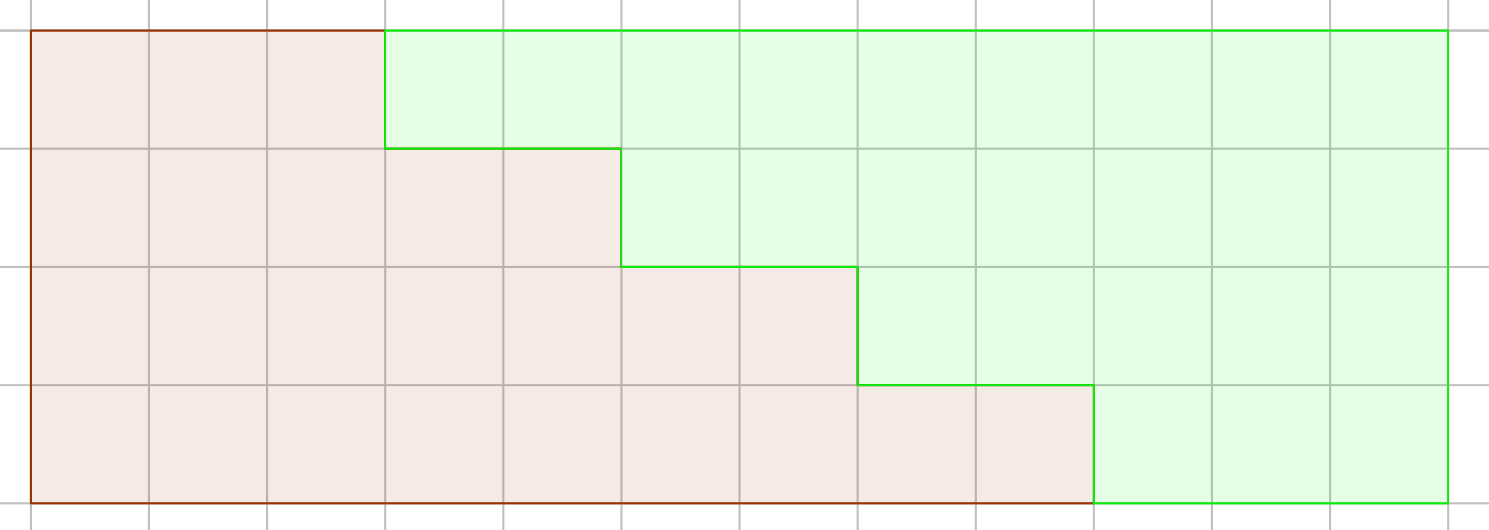
\includegraphics[width=0.5\textwidth]{seriearithmetique}
\]
\begin{theoreme}[Rappel de première, à connaître]
Pour tout $n\in\N^*$,
 \[
  1+2+3+\cdots+n=\frac{n(n+1)}{2}.
 \]
\end{theoreme}
\begin{demonstration}
 On applique le théorème précédent aux $n$ permiers
termes de la suite arithmétique de terme initial 1 et de raison 1.
\end{demonstration}

\begin{theoreme}
Soit $q$ un réel distinct de 1,
 \[
  \sum_{k=0}^{n}q^n=1+q+q^2+\dots+q^n=\frac{1-q^{n+1}}{1-q}.
 \]
\end{theoreme}
\begin{demonstration}
 Pour tout réel $q$, on a :
\begin{align*}
 (1-q)(1+q+q^2+\dots+q^n)&=1+q+q^2+\dots+q^n-q-q^2-q^3-\dots-q^{n+1}\\
			 &=1-q^{n+1}.
\end{align*}
Donc si $q$ est différent de 1, on divise les deux membres par $1-q$
qui est bien différent de 0 pour obtenir le théorème.
\end{demonstration}
\begin{theoreme}[Somme de termes consécutifs d'une suite géométrique]
Dans les hypothèses de la définition d'une suite géométrique, si $q$ est différent de 1
on a :
 \[
  \sum_{k=n}^{p}u_k=u_n+u_{n+1}+\dots+u_{p}=u_n\frac{1-q^{p-n+1}}{1-q}.
 \]
\end{theoreme}
\begin{demonstration}
 En utilisant l'expression du terme général, puis en factorisant, on obtient :
\begin{align*}
 u_n+u_{n+1}+u_{n+2}\dots+u_{p}&=aq^n+aq^{n+1}+aq^{n+2}+\dots+aq^p\\
			&=aq^n(1+q+q^2\dots+q^{n-p})\\
			&=u_n(1+q+q^2\dots+q^{n-p}),
\end{align*}
et le théorème précédent donne la conclusion.
\end{demonstration}

\begin{exercice}
 On emprunte \numprint{100000}\euro{} sur 10 ans à 5\%.
Chaque année, on rembourse la même annuité $a$.
\begin{enumerate}
 \item Justifier que l'on a : $\numprint{100000}=a\times\dfrac{1}{1,05}+a\times{\left(\dfrac{1}{1,05}\right)}^2+\cdots+a\times{\left(\dfrac{1}{1,05}\right)}^{10}$.
 \item Déterminer $a$, en déduire $10\times a$. Expliquez pourquoi ce dernier calcul n'a pas de sens.
\end{enumerate}

\end{exercice}

\begin{exercice}
43 et 44 p. 34, 75 p. 37 (exprimer $u_n$ en fonction de $n$), 47 p. 34.
\end{exercice}

\subsection{Variations}
\begin{definition}[Suite croissante]
 Lorsque la suite $(u_n)_{n\in\N}$ est telle que pour tout $n\in\N$, $u_n\leq u_{n+1}$,
on dit qu'elle est croissante.
\end{definition}
La définition de décroissante est obtenue en chageant le sens de l'inégalité. Dans l'un ou l'autre
cas, on dit que la suite est monotone.
Lorsque les inégalités
sont strictes on peut parler de suite strictement croissante (ou décroissante). 
Lorsque l'inégalité n'est vérifiée
qu'à partir d'un certain rang, on parle de suite (strictement) croissante (ou décroissante) à partir 
de ce rang.
\begin{theoreme}
 Soit $f$ une fonction définie sur $\R^+$ et $(u_n)_{n\in\N}$ la suite définie par $u_n=f(n)$.
Si $f$ est (strictement) monotone sur $\R^+$, $(u_n)$ est monotone, de même monotonie (stricte). 
\end{theoreme}
\begin{demonstration}
 Dans le cas o\`u $f$ est croissante sur $\R^+$. Soit $n\in\N$, on a :
\begin{align*}
 0\leq n&<n+1,\\
  \text{donc }f(n)&\leq f(n+1)\text{ car $f$ est croissante sur $\R^+$, et donc :}\\
  u_n&\leq u_{n+1}.
\end{align*}
Les autres cas se démontrent de la même façon.
\end{demonstration}
\begin{theoreme}[Deux reformulations utiles de la monotonie]
\begin{enumerate}
 \item Pour tout $n\in\N$, $u_n\leq u_{n+1}$ $\equi$ Pour tout $n\in\N$, $u_{n+1}-u_n\leq0$.
 \item Pour tout $n\in\N$, $0<u_n\leq u_{n+1}$ $\equi$ Pour tout $n\in\N$, $u_n>0$ et $\dfrac{u_{n+1}}{u_n}\geq1$.
\end{enumerate}
\end{theoreme}

\begin{exercice}
 \begin{itemize}
  \item Montrer que la suite géométrique $(u_n)$ de premier terme $u_0=5$ et de raison $\dfrac12$ est
  décroissante.
  \item Montrer que la suite géométrique $(v_n)$ de premier terme $u_0=1$ et de raison $3$ est
  croissante.
 \end{itemize}
\end{exercice}

\begin{exercice}[D'après Amérique du Nord, mai 2013]
 Soit $(u_n)$ la suite définie par $u_0=1$ et pour
 tout $n\in\N$, $u_{n+1}=\sqrt{2u_n}$.
 \begin{enumerate}
  \item Montrer que pour tout $n\in\N$, $0<u_n\leq2$.
  \item Déterminer le sens de variation de la suite $(u_n)$.
 \end{enumerate}

\end{exercice}


\begin{exercice}[D'après Liban, mai 2013]
 Soit $(v_n)$ la suite définie par $v_0=1$ et pour
 tout $n\in\N$, $v_{n+1}=\dfrac{9}{6-v_n}$.
 \begin{enumerate}
  \item Montrer que pour tout $n\in\N$, $0<v_n<3$.
  \item Démontrer que pour tout entier naturel $n$, $v_{n+1}-v_n = \dfrac{\left(3-v_n\right)^2}{6-v_n}$.
  La suite $(v_n)$ est-elle monotone ?
 \end{enumerate}
\end{exercice}


\subsection{Suites majorées, minorées, bornées}
\begin{definition}[Suite majorée, minorée, bornée]
 \begin{align*}
  (u_n)_{n\in\N}\text{ majorée}&\equidef\text{ Il exite un nombre réel $M$ plus
 grand que tous les termes de la suite.}\\
  (u_n)_{n\in\N}\text{ minorée}&\equidef\exists m\in\R,\,\forall n\in\N,\,u_n\geq m.\\
(u_n)_{n\in\N}\text{ bornée}&\equidef(u_n)_{n\in\N}\text{ est majorée et minorée.}
\end{align*}
\end{definition}
\begin{exemple}
 La suite $(u_n)$ définie sur $\N^*$ par $u_n=1-\dfrac1{n^2}$ est majorée. Elle est minorée.
Elle est bornée.
\end{exemple}

\begin{exemple}
 La suite $(v_n)$ définie sur $\N$ par $u_n=100+(n-50)^2$ est minorée. Elle n'est pas majorée.
Elle n'est pas bornée.
\end{exemple}

\begin{exercice}
 53 et \textbf{54} p. 34, 58 p. 35.
\end{exercice}

\pagebreak

\section{Axiome de récurrence}
\begin{exemple}[introductif]
 Tours de Hanoï.
\end{exemple}


\label{axiome}
\subsection{Enoncé}
Pour la culture, une version de l'axiome de récurrence qui permet de le voir comme un constituant de la définition de $\N$ :
\begin{axiome}[de récurrence, énoncé version ensembliste.]
	Soit $A\subset\N$ vérifiant les deux conditions : $\left\{\begin{array}{ll}0\in A\\\forall n\in\N,\quad n\in A\Rightarrow n+1\in A\end{array}\right.$. Alors $A=\N$.
\end{axiome}
Ceci doit vous paraître évident et naturel. Il faut le comprendre comme une partie de la définition de 
l'ensemble $\N$ qui exprime
que $\N$ \og n'est pas grand\fg{} dans le sens ou il est le plus petit ensemble obtenu par le procédé de comptage :
\[
	\N=\{0, 1, 2, 3, ...\}
\]

Voyons maintenant un axiome de logique fameux, le \latin{modus ponens} :
\begin{axiome}[de logique, \latin{modus ponens}]
 Si on a prouvé la proposition $\mathcal{P}$, et si on a prouvé la proposition $\mathcal{P}\implique\mathcal{Q}$,
alors on a prouvé $\mathcal{Q}$.
\end{axiome}

\begin{exemple}
 Il y en a dans tous vos raisonnements, c'est tellement courant qu'on l'abrège, et qu'au lieu de dire :
\og $\mathcal{P}$, or $\mathcal{P}\implique\mathcal{Q}$, donc $\mathcal{Q}$\fg, on dit :
$\mathcal{P}$, donc $\mathcal{Q}$.

Ainsi, plutôt que : \og le triangle ABC est rectangle en C. Or, si un triangle est rectangle, 
alors le carré de son grand côté égale la somme des carrés de ses petits côtés. Donc $AB^2=AC^2+CB^2$\fg,
on dit \og le triangle ABC est rectangle en C, donc $AB^2=AC^2+CB^2$\fg.
\end{exemple}

L'axiome de récurrence peut être vu comme un axiome de logique qui permet de faire une infinité de \latin{modus ponens}
d'un seul coup :

\begin{axiome}[de logique, axiome de récurrence]
Soit $\mathcal{P}[n]$ une proposition à une variable $n$.
On suppose qu'on a prouvé les propositions :
\begin{description}
 \item $\mathcal{P}[0]$,
 \item pour tout $n\in\N$, $\mathcal{P}[n]\implique\mathcal{P}[n+1]$,
\end{description}
alors on a prouvé la proposition : \og pour tout $n\in\N$, $\mathcal{P}[n]$\fg.
\end{axiome}
La première proposition est appelée l'initialisation, la seconde est appelée l'hérédité,
et la conclusion est appelée la conclusion...
\begin{exemple}
	On considère la suite $(u_n)_{n\in\N}$ définie par $\left\{\begin{array}{ll}
	                                                u_0&=0\\
                                                  u_{n+1}&=2u_n+1
	                                                \end{array}\right.$. 
Le calcul des premiers termes de cette suite donne :
\[
 \begin{array}{c|c|c|c|c}
  u_0	&	u_1	&	u_2	&	u_3	&	u_4\\\hline
  0	&	1	&	3	&	7	&	15
 \end{array}
\]

On note $\mathcal{P}[n]$ la proposition \og$u_n=2^n-1$\fg. Examinons la véracité de $\mathcal{P}[n]$
selon les valeurs de $n$ :
\begin{itemize}
  \item $\mathcal{P}[0]$ est vraie car : $u_0 = 0$ et $2^0-1=0$.
  \item $\mathcal{P}[1]$ est vraie car : $u_1 = 1$ et $2^1-1=1$.
  \item $\mathcal{P}[2]$ est vraie car : $u_2 = 3$ et $2^2-1=3$.
  \item $\mathcal{P}[3]$ est vraie car : $u_3 = 7$ et $2^3-1=7$.
  \item $\mathcal{P}[4]$ est vraie car ...
\end{itemize}
Comment conclure \og$\forall n\in\N$, $\mathcal{P}_n$ est vraie\fg? La suite est définie par récurrence,
on peut tenter un raisonnement par récurrence.
\end{exemple}

\subsection{Modèle de rédaction}
Notons $\mathcal{P}[n]$  : \og$u_n=2^n-1$\fg, et raisonnons par récurrence.
\begin{enumerate}
    \item Initialisation : Comme $u_0=0$ par définition de $(u_n)$ d'une part, et comme $2^0-1=0$ d'autre part, on a bien $u_0=2^0-1$ ce qui prouve 
    $\mathcal{P}[0]$.
     \item Hérédité : Soit $n\in\N$. Supposons que $\mathcal{P}[n]$ soit vraie. On a donc :
    \[
	    u_n=2^n-1.
    \]
    Or, par définition de $(u_n)$, on a $u_{n+1}=2u_n-1$. On en déduit :
    \[
	    u_{n+1}=2(2^n-1)+1=2^{n+1}-2+1=2^{n+1}-1.
    \]
    On a prouvé $\mathcal{P}[n+1]$, ce qui prouve l'hérédité.
    \item Conclusion : par récurrence\footnote{C'est à ce moment que l'on fait référence à l'axiome de récurrence},
   on a : $\forall n\in\N,\quad \mathcal{P}[n]$, autrement dit $\forall n\in\N,\quad u_n=2^n-1$.
\end{enumerate}

\begin{exercice}
 30 p. 31, 33 p. 32 (basiques), 39 p. 33 (initialisation à n=7), 41 p. 33 (vrai).
\end{exercice}




\pagebreak
\section{Limites}
\subsection{Suites convergentes}
\begin{definition}
 Soit $(u_n)$ une suite numérique réelle et $\ell$ un réel. Lorsque tout intervalle ouvert contenant $\ell$
contient tous les termes de la suite à partir d'un certain rang, on dit que $(u_n)$ converge vers $\ell$ et
on note :
\[
 \lim_{n\to+\infty}u_n=\ell.
\]
\end{definition}
\begin{exemple}
 On a $
 \lim 5+\frac{1}{n}=5.
$
Mais considérons la suite $(u_n)_{n\in\N^*}$ définie par \[
 u_n=5+\frac{1}{n}+(10^{-9}+(-1)^n\times 10^{-9}).
\]
Elle ne ne converge pas : lorsque $n> 10^{10}$, le neuvième chiffre après la virgule alterne entre
0 et 2 : les termes de la suite ne peuvent pas tous être dans aucun intervalle ouvert
de diamètre plus petit que $10^{-9}$ par exemple.
\end{exemple}


\subsection{Suites tendant vers $+\infty$ ou $-\infty$.}
\begin{definition}
 Soit $(u_n)$ une suite numérique. Lorsque tout intervalle de la forme $]A;+\infty[$
 contient toutes les valeurs $u_n$ à partir d'un certain rang, on dit que $(u_n)$ tends vers $+\infty$ et on note :
\[
 \lim_{n\to+\infty}u_n=+\infty.
\]
\end{definition}

\begin{definition}
 Soit $(u_n)$ une suite numérique. Lorsque tout intervalle de la forme $]-\infty;A[$
 contient toutes les valeurs $u_n$ à partir d'un certain rang, on dit que $u_n$ tends vers $-\infty$ et on note :
\[
 \lim_{n\to+\infty}u_n=-\infty.
\]
\end{definition}

\begin{theoreme}[Admis, peut être pris comme axiome]
Une suite numérique réelle croissante et majorée converge dans $\R$.
\end{theoreme}
\begin{remarque}
 L'énoncé : \og une suite numérique rationnelle croissante et majorée converge dans $\Q$\fg{} est
faux. Par exemple, si $(u_n)$ est la suite des approximations décimales à $10^{-n}$ près de
$\sqrt{2}$ c'est une suite croissante majorée de décimaux donc de rationnels, qui converge mais pas
dans $\Q$ : dans $\R$.
\end{remarque}

De manière analogue, une suite décroissante et minorée converge dans $R$.
\begin{theoreme}
 Une suite croissante non majorée tend vers $+\infty$.
\end{theoreme}
\begin{demonstration}[à connaître]
 Soit $(u_n)$ une suite croissante non majorée. Soit $A$ un réel. Comme $A$ n'est pas un majorant
de $(u_n)$, il existe un rang $n_0$ tel que $u_{n_0}$ soit strictement supérieur à $A$. 
Comme $(u_n)$ est croissante, à partir du rang $n_0$ tous les termes de
$(u_n)$ sont supérieurs à $u_{n_0}$ et donc strictement supérieurs à $A$. On a bien démontré que $(u_n)$ tends vers 
$+\infty$, puisque pour tout nombre réel $A$, on a déterminé un rang à partir duquel tous les termes de
la suite sont dans l'intervalle $]A,+\infty[$.
\end{demonstration}
On démontre bien sûr de manière analogue qu'une suite décroissante minorée tend vers $-\infty$.
\begin{exemple}
 Une suite bornée qui ne converge pas : $u_n=(-1)^n$.
\end{exemple}
\begin{exemple}
 Une suite strictement croissante qui ne tend pas vers $+\infty$ : $u_n=1-\dfrac1n$.
\end{exemple}
\begin{exemple}
 Une suite non majorée qui ne tend pas vers $+\infty$ : $u_n=(-1)^nn$, ou $u_n=(-2)^n$.
\end{exemple}

\begin{exercice}
 66 et 67 p. 36, 79 p. 37.
\end{exercice}


\subsection{Limites admises de référence}
\begin{theoreme}[Admis]
 \begin{enumerate}
  \item Pour tout entier $k$ supérieur à 1, $\displaystyle\lim_{n\to+\infty}n^k=+\infty$.
  \item $\displaystyle\lim_{n\to+\infty}\sqrt{n}=+\infty$.
  \item Soit $q$ un réel, alors :
      \begin{enumerate}
	\item si $\abs{q}<1$, alors $\displaystyle\lim_{n\to+\infty}q^n=0$,
	\item si $q>1$, alors $\displaystyle\lim_{n\to+\infty}q^n=+\infty$.
      \end{enumerate}
 \end{enumerate}
\end{theoreme}

\begin{exercice}
 86 p. 38.
\end{exercice}


\subsection{Opérations et limites}
On note $0^+$ la limite 0 par valeurs positives (la suite tend vers 0 et 
est positive à partir d'un certain rang) et $0^-$ la limite 0 par valeurs négatives.
\begin{theoreme}[Admis]
\begin{enumerate}
 \item Le passage à la limite commute avec les opérations sur les nombres réels
lorsqu'elles sont définies.
  \item Lorsqu'elles ne sont pas définies, elles commutent dans les cas suivant avec les conventions de prolongement :
  \begin{enumerate}
   \item Pour tout réel $\ell$,\begin{align*}
	  \ell+\infty&=+\infty,&\ell-\infty&=-\infty,&\frac{\ell}{+\infty}=\frac{\ell}{-\infty}&=0.
	  \end{align*}
   \item Pour tout réel $\ell>0$, ou pour $\ell=+\infty$ :\begin{align*}
	  \ell+(+\infty)&=+\infty,&\ell\times(+\infty)&=+\infty,&\ell\times(-\infty)&=-\infty,
			  &\frac{\ell}{0^+}&=+\infty,&\frac{\ell}{0^-}&=-\infty.
	  \end{align*}
    \item Pour tout réel $\ell<0$, ou pour $\ell=-\infty$ :\begin{align*}
	  \ell+(-\infty)&=-\infty,&\ell\times(+\infty)&=-\infty,&\ell\times(-\infty)&=+\infty,
			  &\frac{\ell}{0^+}&=-\infty,&\frac{\ell}{0^-}&=+\infty.
	  \end{align*}
  \end{enumerate}
  \item On ne peut pas adopter de convention pour les cas suivants :
    \begin{align*}
    +\infty-\infty&&0\times\infty&&\frac{\infty}{\infty}&&\frac{0}{0}
\end{align*}
\end{enumerate}
\end{theoreme}

\begin{exercice}
 68, \textbf{69}, 71, 72 p. 36, 73 et 75 p. 37.
\end{exercice}


\subsection{Comparaison et limites}
\begin{theoreme}[admis, théorème \og des gendarmes\fg]
 Soit $(a_n)$, $(b_n)$ et $(u_n)$ trois suites, et $\ell$ un réel tels que :
\begin{enumerate}
 \item \`A partir d'un certain rang, $a_n\leq u_n\leq b_n$.
 \item $\displaystyle\lim a_n=\lim b_n=\ell$.
\end{enumerate}
Alors $\displaystyle\lim u_n=\ell$.
\end{theoreme}

\begin{exercice}
 81 p. 37.
\end{exercice}

\begin{theoreme}[Preuve exigible]
 Si $(u_n)$ et $(v_n)$ sont deux suites telles que :
\begin{itemize}
  \item à partir d'un certain rang, $u_n\leq v_n$,
  \item la suite $(u_n)$ tend vers $+\infty$,
\end{itemize}
alors la suite $(v_n)$ tend vers $+\infty$.
\end{theoreme}

\begin{demonstration}
 Supposons que $(u_n)$ et $(v_n)$ sont deux suites telles que :
\begin{itemize}
  \item à partir d'un certain rang, $u_n\leq v_n$,
  \item la suite $(u_n)$ tend vers $+\infty$.
\end{itemize}
Il faut prouver que $(v_n)$ tend vers $+\infty$, autrement dit que
tout intervalle de la forme $]A;+\infty[$ contient toutes les valeurs $v_n$ à partir d'un certain rang.
Soit $A$ un réel. Il existe un rang $n_0$ à partir duquel toutes les valeurs $u_n$ sont dans $]A,+\infty[$.
Et d'après la première hypothèse, il existe un rang $n_1$ à partir duquel $u_n\leq v_n$. Donc à partir 
du plus grand des deux rangs $n_0$ et $n_1$, on a bien que tous les termes $v_n$ sont dans $]A,+\infty[$.
\end{demonstration}

\begin{exercice}
 80 p. 37.
\end{exercice}



\begin{theoreme}[Preuve exigible]
 Si une suite est croissante et admet pour limite le réel $\ell$, alors tous les termes de la suite sont inférieurs ou égaux à $\ell$.
\end{theoreme}

\begin{demonstration}
 Soit $(u_n)$ une suite croissante admettant pour limite le réel $\ell$. Il faut prouver que pour tout $n\in\N$, $u_n\leq \ell$.
Par l'absurde, supposons qu'il existe $n_0\in\N$ tel que $u_{n_0}>l$. Alors l'intervalle ouvert $]\ell-1,u_{n_O}[$ contient $\ell$,
mais, comme $(u_n)$ est croissante, il ne peut contenir des termes $u_n$ que pour $n\leq n_0$, ce qui contredit que la limite de $(u_n)$
soit $\ell$.
\end{demonstration}

\begin{exercice}
 117 p. 46 (convergence et monotonie de la somme des termes d'une suite). 
\end{exercice}

TODO : annales de bac.







\end{document}
